\chapter{François-Xavier avant le Concile de Trente}


\section{Contexte}

\paragraph{Rappel du latin appliqué aux chinois par André de Pérouse}



\section{Aux Compagnons vivants à Rome}
\mn{(EX.I, 160-177; S.11, 406-410)}

\textit{Cette longue lettre présente le grand intérêt de nous présenter
plusieurs aspects du choc spirituel et culturel que fut la rencontre
du monde indien et de la Chrétienté occidentale. En arrivant sur
la Côte du Dekkan, saint François Xavier fut frappé par l'ignorance
religieuse de ceux qu'un baptême sans doute hâtif avait rendus
Chrétiens : au Cap Comorin, les atavismes et les traditions hindoues résistent bien chez les néophytes. Comment parvenir à les
couper complètement et de leurs concitoyens hindous et de leur
passé ? Telle est bien la question que se pose l'Apôtre de l'Asie.
La solution par lui trouvée peut paraître « médiévale » ou au
contraire d'une inquiétante « modernité » selon l'idée que chacun
se fait de la marche de l'histoire humaine. Sur lequel de ces deux
versants doit-on placer une institution aussi importante que l'Inquisition
? Et ce que Xavier organise ? Il fait encadrer la population
par un réseau dense de militants, de responsables et même d'agents
de renseignement, fait surveiller les parents par leurs enfants, entreprend
de casser la transmission des usages et des croyances en
tablant sur la jeune génération contre l'ancienne. Ne sommes-nous
pas en terrain connu, celui de la guerre subversive ? S'il veutfaire
du passé table rase, c'est évidemment parce qu'il en a une bien
mauvaise opinion. Selon lui, il n'y a rien de bon à tirer de la religion
païenne qu'il définit comme étant un mélange de satanisme,
d'ignorance et de crédulité. Les Brahmanes ne valent rien. Rien ici
ne préfigure ce qui sera plus tard l'attitude de la Compagnie de
Jésus envers les civilisations asiatiques, Robert de Nobili ou Matthieu
Ricci. La sincérité de Xavier et la chaleur avec laquelle il évoque
à la fin son amitié pour ses Frères ne manquent pas de racheter
son antipathie envers l'Inde, sa caste sacerdotale et sa culture}


\begin{Synthesis}
La première lettre montre la méthode de la \textit{table rase} : extraction de la culture (tout étant considéré comme démon). Apprentissage du latin (? Vérifier car traduction). Mais en tout cas le missionnaire ne fait pas d'effort d'acculturation.
Est ce lié au point de vue missionnaire ou à des cultures "simples"
\end{Synthesis}

\begin{quote}
Cochin, le 15 janvier 1544
+
Ihus ,
La grâce et l'amour du Christ notre Seigneur soient toujours en
notre aide et en notre faveur. Amen.


1. Voici deux ans et neuf mois que je suis parti du Portugal et
depuis, de mon côté, je vous ai écrit trois fois, en comptant cette
lettre-ci ; je n'ai reçu de vous que quelques-unes depuis que je me
trouve ici, en Inde ; elles ont été écrites le 13 janvier de l'année
1542 et Dieu notre Seigneur sait la consolation que j'en ai reçue.
Il doit y avoir deux mois qu'on me les a remises ; si elles sont arrivées
si tard en Inde; c'est parce que le navire qui les transportait
a hiverné à Mozambique.
\begin{Synthesis}
 FX voit que les Comorins sont chrétiens mais n'ont pas de connaissance chrétienne, ni de la foi ni de ce que cela change pour eux. Le premiere chose est de traduire les principales prières chrétiennes et le credo.  
 Par les enfants,
\end{Synthesis}

2. Messire Paul, François de Mansilhas et moi, nous sommes en
bonne santé. Messire Paul se trouve à Goa, au collège de Sainte
Foi, où il a la charge des étudiants de cette maison. François de
Mansilhas et moi, nous sommes parmi les Chrétiens du Cap Comorin.
Voici plus d'un an que je suis chez ces Chrétiens, \mn{saut de page p. 103}à propos desquels
je dois vous dire qu'ils sont nombreux et qu'il se fait chaque jour
beaucoup de nouveaux Chrétiens. Sitôt arrivé sur cette côte
où ils habitent, J'ai tâché de savoir d'eux quelle·connaissance ils
ont du Christ notre Seigneur ; à propos des \textbf{articles de foi}, je leur
ai demandé ce qu'ils croient, \textbf{ou ce qu'ils ont de plus maintenant
qu'ils sont chrétiens que lorsqu'ils étaient païens et je n'ai pas
trouvé d'autre réponse sur leurs lèvres que ceci, à savoir qu'ils sont
chrétiens et qu'eux ne comprenant pas notre langue, ils ne connaissent
pas notre LOI, ou ce qu'il faut croire.} Comme ils ne me comprenaient
pas, et que moi non plus, je ne les comprenais pas, parce
que leur langue paternelle est le malabar et la mienne le biscaien, Je rassemblai ceux d'entre eux qui sont les plus instruits et
Je cherchai des personnes comprenant notre langue et la leur.
Après nous être à grand peine réunis de longs jours durant nous
avons traduit les prières, tout d'abord la façon de faire le signe de
croix en confessant que les trois Personnes sont un seul Dieu ;
ensuite, le Credo, les commandements, le Pater Noster, l'Ave
Maria, le Salve Regina et la confession générale, de latin en malabar.
Après les. avons traduites dans leur langue et les avoir apprises
par coeur, Je m'en suis allé par tout le village 4 une cloche à la
main, pour rassembler tous les enfants et tous les hommes que je
pouvais réunir. Une fois assemblés, je les ai instruits deux fois par
Jour. Je leur ai enseigné les prières pendant la durée d'un mois leur
ayant donné cet ordre que les enfants enseigneraient à leurs ~ères
et mères,et à tous ceux de leur maison et de leur voisinage ce qu'ils
ont appris à l'école.
\begin{Synthesis}
enseignement du Credo comme coeur de la foi. A la différence des Nestoriens, qui partent de l'histoire du Christ et de la loi, ici, importance de la foi.
Puis la Loi de Jesus Christ (10 commandements), conforme à la raison naturelle. La pratique vient donc après l'annonce de la fois. 
\end{Synthesis}
3. Le dimanche, j'assemblais tous les habitants du village, hommes
aussi bien que femmes;°les, grands et petits, pour réciter les prières
dans leur langue ; ils y ont montré beaucoup de plaisir et ils
Y sont venus avec beaucoup d'allégresse. Après avoir commencé
par confesser un seul Dieu, trine et un, ils ont récité le Credo à
Pleine voix dans leur langue et au fur et à mesure que je le leur ai
~eclté tous m ont donné les réponses. Une fois le Credo terminé,
Je le reprenais tout seul ; disant chaque article séparément et
m'arrêtant à chacun des douze, je les admonestais en leur expliquant que le nom de « Chrétiens » ne signifie rien d'autre que de
croire fermement et sans doute aucun ces douze articles ; puisqu'ils
ont proclamé qu'ils sont chrétiens, je leur demandais s'ils croient
fermement en chacun de ces douze articles. De la sorte, tous ensemble \mn{Saut de page p. 104} à pleine voix, hommes et femmes, grands et petits me répondaient
à chaque article que oui, les bras posés l'un sur l'autre sur
la poitrine, à la façon d'une croix ; je leur ai fait de la sorte réciter
le Credo plus souvent que n'importe quelle autre prière, puisque
c'est seulement en croyant à ces douze articles qu'on peut
s'appeler chrétien. Après le Credo, la première chose que je leur
enseigne est les commandements, en leur disant que la Loi des
Chrétiens en contient seulement dix et qu'on peut dire de quelqu'un
qu'il est un bon chrétien s'il les observe comme Dieu l'ordonne,
et qu'au contraire il est un mauvais chrétien s'il ne les observe pas.
Les Chrétiens aussi bien que les Gentils sont très frappés de voir
combien sainte et conforme à toute raison naturelle est la Loi de
Jésus-Christ. Une fois terminés le Credo et les commandements,
je dis le Pater Noster et l' Ave Maria et à mesure que je les récite
tous me répondent. Nous récitons douze Notre Père et douze Ave
Maria en l'honneur des douze articles de foi et, une fois terminés,
nous disons dix autres Notre Père avec dix Ave Maria, en l'honneur
des dix commandements, le tout en observant l'ordre qui suit.
Nous disons d'abord le premier article de la foi et quand nous
avons fini de le dire, je dis en leur langue, et eux avec moi :
\begin{quote}
    « Jésus-Christ, Fils de Dieu, donnez-nous la grâce de croire fermement,
et sans doute aucun, le premier article de la foi » ;
\end{quote}
 et pour
qu'il nous donne cette grâce, nous récitons un Pater Noster. Une
fois terminé le Pater Noster, nous disons tous ensemble : \begin{quote}
    « Marie,
mère de Jésus-Christ, obtenez-nous la grâce de votre Fils JésusChrist
pour que nous croyions fermement, et sans doute aucun, le
premier article de la foi» ;
\end{quote} pour qu'elle nous obtienne cette grâce,
nous lui disons l' Ave Maria. Nous suivons le même ordre dans tous
les onze autres articles.

\begin{Synthesis}
Croire fermement : on n'a pas besoin d'une \textit{traduction culturelle} "un et trine". Mais en fait, on croit à l'envoyé mais croit on aux paroles ? 

\end{Synthesis}

4. Une fois terminés le Credo et les douze Pater Noster et Ave
Maria comme je l'ai dit, nous récitons les commandements selon
l'ordre suivant: d'abord, je dis le premier commandement et tous
le disent comme moi; et après qu'ils ont fini de le dire, nous disons
tous ensemble: « Jésus-Christ, Fils de Dieu, donnez-nous la grâce
de vous aimer par-dessus toutes les choses. » Une fois cette grâce
demandée nous disons tous le Pater Noster ; et une fois terminé
celui-ci , nous disons : « Sainte Marie, Mère de Jésus-Chris. t,
obtenez-nous de votre Fils la grâce de pouvoir observer le premier
commandement. » Une fois cette grâce demandée à Notre Dame
nous disons tous l' Ave Maria. Nous suivons ce même ordre pour
tous les neuf autres commandements. Si bien qu'en honneur des
douze articles de la foi nous récitons douze Pater Noster avec douze
Ave Maria, en priant Dieu notre Seigneur de nous donner \mn{Saut de page p. 105} la grâce de les observer. Telles sont les demandes que je leur enseigne
à faire par nos prières, en leur expliquant que s'ils obtiennent
ces grâces de Dieu notre Seigneur, il leur donnera tout le reste avec
plus de prodigalité qu'ils ne sauraient le demander. Je fais réciter
à tous la confession générale, et spécialement à tous ceux qui vont
être baptisés, et ensuite le Credo. Quand après les avoir interrogés
sur chaque article pour leur demander s'ils croient fermement
et qu'ils me répondent que oui, et que je leur ai dit ce qu'est la Loi
de Jésus-Christ qu'ils doivent observer pour être sauvés, je les baptise.
Nous récitons le Salve Regina quand nous voulons terminer
nos prières.

\begin{Synthesis}
Rôle des jeunes :  acte d'espérance qu'ils corrigent leur parents.
\end{Synthesis}

5. J'espère en Dieu notre Seigneur que les enfants deviendront
de meilleures gens que leurs parents, car ils montrent beaucoup
d'amour et de bonne volonté envers notre Loi, ainsi que pour
apprendre les prières et les enseigner. Ils éprouvent une grande horreur
pour les idolâtries des Gentils, au point que, souvent, ils se
battent avec les Gentils et qu'ils réprimandent leurs pères et mères
quand ils les voient adorer les idoles ; ils les dénoncent en venant
me le dire et quand ils m'informent de telle ou telle idolâtrie qui
se fait en dehors du village, je rassemble tous les jeunes du village
et je m'en vais avec eux à l'endroit où on a fait des idoles. Alors
le diable reçoit de ces enfants venus avec moi plus d'outrages qu'il
n'a reçu d'honneurs de la part de leurs pères, mères et personnês
apparentées au moment où ils dressent et adorent ces idoles. Ces
enfants se saisissent en effet des idoles et les mettent en miettes
aussi menues que cendre ; ensuite, ils crachent dessus, les foulent
aux pieds et font ensuite dessus d'autres choses ; quoiqu'il ne semble
pas bien de les appeler par leur nom, c'est tout à l'honneur de
ces enfants de les faire sur celui qui a la si grande audace de se faire
adorer par leurs parents. J'ai vécu dans une localité importante et
peuplée de Chrétiens pour traduire les prières de notre langue dans
la leur et pour les enseigner pendant quatre mois.

\begin{Synthesis}
FX détruit les idoles. Théologie deutéronomiste . Mais comme on ne maitrise pas la langue de l'autre, il n'y a que les actes, et quels actes n'ont plus de valeur que de détruire les idôles pour représenter la foi, \textit{le zèle ardent} ?

Autre acte : la sollicitude pour les malades et la prière, qui se fait via les enfants, \textit{envoyés de FX} auprès des malades. 
\end{Synthesis}
6. Durant.cette période, ils ont été très nombreux à venir me
chercher pour que j'aille chez eux réciter des prières sur les malades
et sur les autres qui sont venus me chercher avec leurs maladies.
Ils ne me laissaient pas un instant de repos ou sans avoir
d'occupation, en dehors de la récitation des Evangiles, de l'enseignement
des enfants, de leur baptême et des traductions, sans
compter la sépulture de ceux qui meurent. C'était au point que,
pour répondre à la dévotion de ceux qui me faisaient venir ou qui
venaient me chercher, j'avais trop d'occupations. Mais, pour qu'ils
ne perdissent point la confiance qu'ils ont envers notre religion et
notre Loi chrétiennes, il ne m'était pas possible de refuser une si
\mn{Saut de page p.106} pieuse demande. Comme la chose s'accroissait démesurément et
que je ne pouvais tous les satisfaire, j'ai donné l'ordre aux enfants
qui savaient les prières d'aller chez les malades et de réunir tous
ceux de la maisonnée et du voisinage, et de leur dire tous le Credo
bien des fois, en disant au malade de croire et qu'il serait guéri ;
et ensuite les autres prières. De la sorte, j'ai satisfait tout le monde
et j'ai fait réciter dans les maisons et sur les places le Credo, les
commandements et les autres prières. Ainsi, Dieu notre Seigneur
leur accorde de grandes grâces en même temps que la santé spirituelle
et corporelle aux malades, de par la foi de la maisonnée, du
voisinage ou par la leur propre. Dieu s'est servi d'une grande miséricorde
envers ceux qui souffraient, car c'est par les maladies elles-mêmes
qu'il les a appelés et qu'ils les a amenés à la foi presque de
force .


7. Après avoir laissé dans ce village quelqu'un qui poursuive ce
qui a été commencé, je suis en train de visiter les autres villages
pour faire la même chose ; c'est pourquoi jamais les pieuses et saintes
occupations ne me font défaut en ce pays. Je n'en aurais jamais
fini si je voulais décrire le fruit qu'on recueille en baptisant les
enfants qui naissent et en enseignant ceux qui en ont l'âge requis.
Dans les localités que je traverse, je laisse par écrit les prières et,
à ceux qui savent écrire, je donne ordre de les écrire et de les
apprendre par coeur et de les réciter tous les jours ; j'ordonne aussi
à tous de se réunir le dimanche pour les réciter. Dans ce but, je
laisse dans les villages quelqu'un qui en aura la charge.

\begin{Synthesis}
C'est les bras fatigués devant tout le travail. Et le caractère vain des études de théologie quand les ouvriers sont si peu nombreux. Une vraie question que je reçois. 
Quelle conversion quand on voit le rôle du gouverneur et de ces 4000 pièces d'or.
\end{Synthesis}

8. C'est un grand nombre de nouveaux Chrétiens qu'on se prive
de faire en ce pays, faute d'avoir des personnes pour se consacrer
à de si pieuses et si saintes choses. Bien souvent, l'idée me prend
d'aller aux lieux où, chez vous, on étudie, pour y crier comme un
homme qui a perdu le jugement, et surtout à l'université de Paris ;
je dirais à la Sorbonne à ceux qui ont plus de science que de
volonté pour se préparer à en tirer du fruit : \begin{quote}
    « Que d'âmes sont
empêchées d'aller à la gloire et vont en enfer par la négligence de
ceux-là ! » 
\end{quote}Si tout comme ils étudient la science, ils étudiaient aussi
le compte que Dieu notre Seigneur en demandera, de cette science
et du talent qu'il leur a donné, beaucoup d'entre eux seraient
émus ; ils recourraient aux moyens et aux exercices spirituels capables
de leur faire connaître et sentir en leurs âmes la volonté divine.
Se conformant davantage à celle-ci qu'à leurs affects personnels,
ils diraient : \begin{quote}
    « Seigneur, me voici ; que voulez-vous que je fasse ?
Envoyez-moi où vous voulez, et, si cela convient, même chez les
Indiens. » Comme ils vivraient beaucoup plus consolés! Ils
auraient une plus grande espérance en la miséricorde divine à
\mn{Saut de page p.107}     l'heure de la mort, quand ils seraient soumis au jugement particulier
auquel personne ne peut échapper, car ils pourraient alléguer
pour eux-mêmes:« Seigneur, vous m'avez donné cinq talents; en
voici quinze autres que j'ai gagnés . »
\end{quote} 
Je crains que beaucoup de
ceux qui étudient dans les Universités n'étudient davantage pour
obtenir par la science des dignités, des bénéfices, des évêchés, plutôt
qu'avec le désir de se conformer aux besoins requis par les dignités
et par les états ecclésiastiques. Ceux qui étudient ont coutume
de dire : « Je désire avoir la science pour obtenir grâce à elle quelque
bénéfice ou dignité ecclésiastique, et ensuite, au moyen de cette
dignité, servir Dieu. » C'est ainsi que suivant leurs affections désordonnées,
ils font leur élection en craignant que Dieu ne veuille pas
ce que eux, ils veulent, car leurs affections désordonnées ne leur
permettent pas de faire cette élection selon la volonté de Dieu notre
Seigneur. Je me suis senti presque poussé à écrire à l'université de
Paris, du moins à notre maître de Cornibus et au docteur Le
Picart, pour leur dire que des milliers et des milliers de Gentils
se feraient chrétiens s'il y avait des ouvriers, pour prendre soin de
chercher et d'aider les personnes qui s'attachent non pas à leurs
propres biens mais à ceux de Jésus-Christ.

Le nombre de ceux
qui, en ce pays où je me déplace, se convertissent à la foi du Christ
est tel que souvent il m'arrive d'avoir les bras fatigués de baptiser
et de ne plus pouvoir parler davantage pour réciter le Credo et les
commandements en leur langue, ainsi que les autres prières, outre
une exhortation que je sais dans leur langue, dans laquelle je leur
explique ce que veut dire être chrétien, ce qu'est le paradis, ce
qu'est l'enfer et où je leur dis quels sont ceux qui vont d'un côté
et quels sont ceux qui vont de l'autre. Plus que toute autre prière,
je leur dis souvent le Credo et les commandements ; il y a des jours
où je baptise tout un village ; et sur cette côte que je parcours, il
y en a trente de Chrétiens. \textit{Le Gouverneur de cette Inde est grand ami de ceux qui se font
chrétiens.} Il a fait don de quatre mille pièces d'or chaque année,
qu'on doit dépenser seulement pour les donner à ces personnes qui,
avec une grande diligence, enseignent la doctrine chrétienne dans
les villages qui se sont convertis récemment à la foi. Il est grand
ami aussi de tous ceux de notre Compagnie ; il souhaite fort que
\mn{Saut de page p. 108}  certains de notre Compagnie viennent en ce pays et il a écrit en ce
sens, me semble-t-il, au Roi.

\begin{Synthesis}
Collège de Goa pour apprendre le latin, permettant aux étudiants de devenir prêtre et missionnaire. 
\end{Synthesis}

9. L'an passé, j'ai écrit à propos d'un collège qu'on fonde dans
la ville de Goa et où il y a déjà beaucoup d'étudiants de diverses
langues, tous nés de parents infidèles. A l'intérieur du collège où
il y a déjà beaucoup de bâtiments construits, il y a parmi eux beaucoup
qui apprennent le latin et d'autres à lire et à écrire. Messire
Paul vit avec les étudiants de ce collège ; il leur dit la messe chaque
jour et il les confesse ; il ne cesse pas un instant de leur donner
de la doctrine spirituelle ; il a aussi la charge de toutes les choses
corporelles nécessaires à ces étudiants. Ce collège est très vaste
et on peut y faire tenir cinq cents étudiants ; il possède des rentes
suffisantes pour les faire vivre. Nombreuses sont les aumônes qui
sont données à ce collège, sans compter que le Gouverneur l'aide
généreusement. C'est chose dont tous les Chrétiens doivent rendre
grâces à Dieu notre Seigneur que la sainte fondation de cette maison
qui est nommée Collège de la Sainte Foi. J'espère en la miséricorde
de Dieu notre Seigneur que, d'ici peu d'années, le nombre
des Chrétiens sera de beaucoup multiplié et que les frontières de
l'Eglise s'élargiront au moyen de ceux qui étudient dans ce saint
collège.

\begin{Synthesis}
Les brahmanes s'opposent à l'évangélisation. Les raisons pour FX sont l'intérêt qu'ils ont pour les offrandes. 
\end{Synthesis}

10. Dans ce pays, il y a parmi les Gentils une engeance qu'on
appelle les Brahmanes. Ce sont eux qui animent toute la Gentilité.
Ils ont la charge des maisons où se trouvent les idoles ; c'est la plus
perverse gent du monde. C'est à eux que s'applique le psaume qui
dit : \begin{quote}
    « Des gens qui ne sont pas saints, de l'homme inique et trompeur,
protège-moi 8 » 
\end{quote}Voici des gens qui ne disent jamais la vérité
et qui ont perpétuellement à l'esprit de trouver comment mentir
avec subtilité et comment tromper les pauvres simples et les ignorants.
C'est ainsi qu'ils leur disent que les idoles demandent qu'on
leur apporte certaines choses en offrande et ces choses ne sont rien
d'autre que celles que les Brahmanes inventent et qu'ils veulent
pour nourrir leurs femmes, leurs enfants et leur maisonnée. Ils font
croire aux simples d'esprit que les idoles mangent et il y a beaucoup
de gens qui, avant de déjeuner ou de souper, offrent une
petite pièce à l'idole. Deux fois par jour, avec grand accompagnement
de timbales, ils mangent, tout en faisant croire à ces malheureux
que ce sont les idoles qui mangent. Lorsque le nécessaire vient
à manquer aux Brahmanes, ceux-ci disent aux gens du peuple que
les idoles sont très en colère contre eux, parce qu'ils ne fournissent
pas les choses qu'elles leur font demander par l'intermédiaire
\mn{Saut de page}  des Brahmanes; s'ils ne les apportent pas, qu'ils prennent bien
garde aux idoles, qui vont les tuer ou leur envoyer des maladies,
ou des démons à domicile. Alors, ces pauvres gens simples d'esprit,
croyant qu'il va en être ainsi, font ce que veulent les Brahmanes,
par crainte que les idoles ne leur fassent du mal.


\begin{Synthesis}
manque d'instruction des brahmanes, signe de la pauvreté de la région. Un seul Brahmane converti.
La foi professée par les brahmanes semble ridicile (ne pas tuer les vaches, donner des aumônes aux brahmanes). 
Parmi les questions, il ne s'agit pas de la conduite des chrétiens mais de la question de la mortalité de l'âme et du corps. 
\end{Synthesis}

11. Ces Brahmanes sont des gens peu instruits. Ce qui leur fait
défaut en matière de vertu, ils le possèdent sans mesure sous forme
d'iniquité et de méchanceté. Les Brahmanes de cette côte que je
parcours voient avec grand déplaisir que je ne fais jamais rien
d'autre que de dévoiler leurs méchancetés ; quand nous nous trouvons
seuls, eux-mêmes me dévoilent la vérité ; et me disent comment
ils trompent le peuple. Ils m'avouent en secret qu'ils n'ont
pas d'autre patrimoine que ces idoles de pierre dont ils vivent en
disant des mensonges.
Ces Brahmanes considèrent que j'en sais plus, moi, qu'eux tous
réunis. Ils m'envoient des délégations et ils sont très chagrinés de
ce que je ne veuille point accepter les présents qu'ils m'envoient.
Ils font tout cela pour que je ne dévoile pas leurs secrets en disant
qu'eux, ils savent bien qu'il n'y a qu'un seul Dieu et qu'ils prieront
Dieu pour moi. Pour récompense de tout cela, je leur dis, de
moi à eux, ce qui me semble et je dévoile leurs tromperies et leurs
sornettes aux pauvres simples qui sont leurs dévots seulement par
crainte, et cela jusqu'à m'en fatiguer. Beaucoup perdent leur dévotion
envers le démon en raison de ce que je leur dis et se font chrétiens.
S'il n'y avait pas les Brahmanes, tous les Gentils se convertiraient
à notre foi. Les maisons où se trouvent les idoles et les
Brahmanes s'appellent des pagodes.
Les Gentils de ce pays sont tous très ignorants ; mais, pour faire
le mal, ils en savent long. Depuis que je suis dans ce pays, je n'ai
fait chrétien qu'un seul Brahmane : c'est un très bon garçon. Il
s'est choisi comme métier d'enseigner aux enfants la doctrine
chrétienne.
\begin{Synthesis}
Vilénie de l'interlocuteur : je le laisse parler. Comme le Christ.
\end{Synthesis}
Sur ma route, lorsque je vais rendre visite aux villages chrétiens,
je passe par de nombreuses pagodes. Je suis une fois passé par une
d'elles où il y avait plus de deux cents Brahmanes qui sont venus
me voir. Parmi les nombreux sujets examinés, je leur ai posé une
question et c'était la suivante : qu'ils me disent ce que leurs dieux
et leurs idoles qu'ils adorent leur ordonnent de faire pour aller à
la gloire. Il y eut alors une grande dispute entre eux pour savoir
qui me répondrait ; ils dirent à l'un des plus anciens de me répondre.
\mn{Saut de page}  Ce vieillard, qui avait plus de quatre-vingts ans, me dit de lui
dire d'abord ce que le Dieu des Chrétiens ordonnait de faire. Moi,
comprenant sa vilenie, je ne voulus rien en dire avant que lui, il
n'en ait d'abord parlé. Il lui fut alors bien forcé de révéler son
ignorance. Il me répondit que leurs dieux ordonnent de faire deux
choses pour aller là · où ils se trouvent : la première est de ne pas
tuer les vaches qu'eux, ils adorent ; la seconde, c'est de donner des
aumônes et celles-ci aux Brahmanes qui sont au service des pagodes.
Après avoir entendu cette réponse, et navré de voir les démons
se rendre maîtres ainsi de nos prochains, démons qui se font adorer
par eux à la place de Dieu, je me suis levé et j'ai dit aux Brahmanes
de rester assis. J'ai alors récité à pleine voix et dans leur langue
le Credo et les commandements de la Loi, en m'arrêtant sur
chacun d'eux. Les commandements achevés, je leur ai fait une
exhortation dans leur langue pour leur expliquer ce qu'est le paradis
et ce qu'est l'enfer, et leur dire qui sont ceux qui vont dans un
endroit et qui sont ceux qui vont dans l'autre. Une fois terminée
cette causerie, les Brahmanes se sont tous levés et m'ont cordialement
embrassé ; ils m'ont dit que vraiment le Dieu des Chrétiens
est un vrai Dieu, car ses commandements sont si conformes à toute
raison naturelle.
Ils m'ont demandé si notre âme meurt en même temps que le
corps, comme celle des bêtes brutes. Dieu notre Seigneur m'a alors
inspiré ces arguments conformes à leur intelligence, tels que je leur
ai fait clairement comprendre l'immortalité des âmes, ce dont ils
montrèrent beaucoup de joie et de plaisir. Les arguments qu'on
doit utiliser auprès de ces gens stupides ne doivent pas être aussi
subtils que ceux qu'on trouve écrits chez les docteurs experts en
scolastique. Ils m'ont demandé: quand un homme meurt, par où
sort son âme? Et quand un homme dort et qu'il rêve qu'il est dans
un pays avec ses amis et ses connaissances (ce qui m'arrive à moi
souvent, de me trouver avec vous, très chers), est-ce que son âme
s'en va là-bas et cesse d'informer son corps? Ils m'ont aussi
demandé si Dieu est blanc ou noir en raison de la diversité des cou.
leurs qu'on trouve chez les hommes. Comme tous ceux de ce pays
sont noirs et que leur couleur leur plaît, ils disent que Dieu est noir
et c'est pourquoi la plupart de leurs idoles sont noires. II les enduisent
souvent d'huile et elles sentent si mauvais que c'est épouvantable.
Elles sont si laides que rien que de les voir on en a peur. A
toutes leurs questions par eux posées, je leur fis des réponses qu'ils
ont trouvées satisfaisantes. Mais quand j'en venais devant eux à
la conclusion qu'ils devaient se faire chrétiens, puisqu'ils connaissaient
la vérité, ils répondaient ce que répondent d'ordinaire
\mn{Saut de page}
    beaucoup d'entre nous : \begin{quote}
        « Qu'est-ce que le monde va dire de nous
si nous faisons un pareil changement d'état dans notre façon de
vivre ? » 
    \end{quote}Sans compter d'autres tentations, en pensant que le nécessaire
viendrait à leur manquer.


\begin{Synthesis}
discussion avec le brahmane \textit{Nicodème} ;) 
Incompréhension entre le brahmane qui fait une distinction entre la foi des érudits et du peuple avec un risque de gnosticisme, et la religion universelle de FX. Importance pour le christianisme d'être transparent et non caché.
\end{Synthesis}

12. Je n'ai trouvé qu'un seul Brahmane, dans un village de la
Côte, à savoir quelque chose, car on me disait qu'il avait étudié
dans des écoles renommées. J'ai voulu avoir une entrevue avec lui
et j'ai trouvé le moyen de nous voir. Il me dit en grand secret que
la première chose que font ceux qui enseignent dans cette école
c'est de faire jurer, à ceux qui viennent s'y instruire, de ne jamais
dire certains secrets qu'ils enseignent. Mais à moi et en grand
secret, ce Brahmane m'a dit ces secrets, en raison de l'amitié qu'il
éprouvait envers moi. Voici un de ces secrets : ne jamais dire qu'il
n'y a qu'un seul Dieu, Créateur du ciel et de la terre, et qui est aux
cieux ; et que lui, il devait adorer ce Dieu, et non pas les idoles
qui sont des démons. Ils possèdent certaines Ecritures qui contiennent
les commandements. La langue qu'on enseigne dans ces écoles
est chez eux comme le latin chez nous. Il me dit très bien les
commandements, chacun d'eux avec une bonne explication. Chose
à peine croyable, ceux qui sont savants observent le dimanche. Et
le dimanche, ils ne récitent qu'une seule oraison, et de nombreuses fois : \begin{quote}
    « Om sri Nardyana Namah »,
\end{quote} ce qui veut dire : « Je
t'adore, ô Dieu, avec ta grâce et avec ton aide, pour toujours 11 »
Et ils récitent cette prière très discrètement et à voix basse, afin de
respecter le serment qu'ils font. Il m'a dit que la loi naturelle leur
défendait d'avoir plusieurs femmes ; ils croient aussi, conformément
à leurs Ecritures, qu'un temps viendra où tous devront vivre
sous une même Loi. Ce Brahmane m'a dit en outre qu'on enseigne
beaucoup d'incantations dans ces écoles.
Il me pria de lui dire les choses··les plus importantes que les Chrétiens
ont dans leur Loi : il me promettait de ne les révéler à personne.
Moi, je lui ai dit que je ne les lui dirais point, à moins qu'il
ne me promît d'abord de ne pas garder secrètes les choses les plus
importantesq ue j'allais lui dire de la Loi des Chrétiens ; il me promit
donc de les rendre publiques 12 Alors, je lui ai dit et je lui ai \mn{Saut de page}
  expliqué avec un grand plaisir ces si importantes paroles de notre
Loi : « Celui qui croira et qui sera baptisé sera sauvé   » Il écrivit
ces mots dans sa langue, avec leur explication, car je lui ai dit
tout le Credo ; dans mon explication, j'ai mis les commandements,
en raison de la conformité qu'il y a entre ceux-ci et le Credo. Il
me dit qu'une nuit, il avait rêvé avec bien du plaisir et de la joie
qu'il allait devenir chrétien, qu'il serait mon compagnon et qu'il
allait me suivre. Il me demanda de le faire chrétien caché, et de
plus sous certaines conditions qui ne sont ni justes ni licites ; c'est
pourquoi je ne les ai pas acceptées. J'espère en Dieu qu'il le deviendra
sans aucune de ces conditions. Je lui ai dit qu'il devait enseigner
aux gens simples à n'adorer qu'un seul Dieu, Créateur du ciel
et de la terre et qui est aux cieux. Mais lui, il n'a pas voulu faire
cela, en raison du serment qu'il avait fait et par crainte d'être tué
par le démon.


13. Je ne vois rien de plus à vous écrire à propos de ce pays, si ce n'est que les consolations communiquées par Dieu notre Seigneur
à ceux qui s'en vont parmi ces Gentils pour les convertir à
la foi du Christ sont si grandes que, s'il existe quelque contentement
en cette vie, on peut dire que c'est celui-ci. Il m'arrive très
souvent d'entendre quelqu'un qui vit parmi ces Chrétiens dire : \begin{quote}
    « 0
Seigneur, ne me donnez pas toutes ces consolations en cette vie !
Ou si vous· me les donnez par votre infinie et miséricordieuse bonté,
emportez-moi donc dans votre sainte gloire ! Car c'est trop de
peine que de vivre sans vous voir, une fois que vous vous êtes ainsi
communiqué intérieurement à vos créatures. »
\end{quote} Oh ! si ceux qui 
cherchent la science consacraient autant d'effort à en tirer profit
qu'ils consacrent de jours et de nuits laborieuses à l'apprendre !
Oh ! si ce contentement que recherche un étudiant dans la compréhension
de ce qu'il étudie, il le cherchait en faisant sentir à ses
prochains ce qui leur est nécessaire pour connaître et pour sentir
Dieu, comme ils se trouveraient plus consolés et mieux préparés
à rendre compte de leur âme, le jour où le Christ lui demandera :
\begin{quote}
    « Rends compte de la manière dont tu as géré mon bien 14 »
\end{quote}

14. Les récréations que j'ai dans ce pays, c'est de me souvenir
bien souvent de vous, mes Frères très chers, et du temps où, par
la grande miséricorde de Dieu notre Seigneur, je vous ai connus
et où j'ai vécu avec vous. Car je sais en moi-même et je sens en
l'intérieur de mon âme, combien, par ma faute, j'ai laissé perdre
de ce temps passé avec vous en ne profitant pas des nombreuses
\mn{Saut de page } connaissances que Dieu vous a communiquées de lui-même. Par
vos prières et par le souvenir continuel que vous avez de me recommander
à lui, Dieu m'accorde une si grande grâce que je sais qu'en
votre absence corporelle, mais par votre faveur et votre aide Dieu
me fait sentir l'infinie multitude de mes péchés et qu'il me donne
la force d'aller chez les infidèles. J'en rends d'abondantes grâces
à Dieu notre Seigneur, ainsi qu'à vous, mes très chers Frères.
Parmi les nombreuses grâces que Dieu notre Seigneur m'a accordées
en cette vie et qu'il me donne tous les jours, il en est une qui
est d'avoir vu de mon vivant ce que j'ai tant désiré à savoir la confirmation
de notre règle et de notre genre de vie. Grâces soient rendues
à Dieu notre Seigneur pour toujours, car il a jugé bon de
manifester publiquement ce qu'il avait fait sentir en secret à son
serviteur Ignace, notre Père.
(L'an passé, je vous ai écrit le nombre des messes que, dans ces
pays des Indes, Messire Paul et moi, nous avons dites pour le Révérend
Cardinal Guidiccioni 15 J'ignore le nombre de celles que
nous avons dites ici depuis un an. Croyez bien que toutes nos messes
sont pour lui. Pour notre consolation, faites-nous savoir combien
Sa Révérendissime Seigneurie se signale dans le service de
Dieu : vous augmenterez également chez Messire Paul et chez moi
le zèle, en sorte que nous devenions ses chapelains perpétuels. Ne
manquez pas de nous écrire sur le fruit qu'il cueille dans l'Eglise.)
Je termine en priant Dieu notre Seigneur de nous réunir à nouveau
dans sa sainte Gloire, puisque dans sa miséricorde il nous a
réunis puis, pour son service, éloignés les uns des autres.



15. Et pour obtenir cette grâce et ce bienfait, prenons pour intercesseurs
et pour avocats toutes ces saintes âmes de ce pays où je
me trouve, âmes que Dieu notre Seigneur a emportées dans sa
sainte gloire après que je les eus baptisées et de ma main et avant
qu'elles ne perdent l'état d'innocence : je crois que· leur nombre
dépasse mille. A toutes ces saintes âmes, je demande qu'elles nous
obtiennent de Dieu notre Seigneur cette grâce, à savoir que pendant
tout le temps où nous serons dans cet exil, nous sentions au dedans
de nos âmes sa très sainte volonté et que nous l'accomplissions
à la perfection.
Votre frère très cher dans le Christ.

François
\end{quote}

\section{Au P. Ignace de Loyola, à Rome 
}
\mn{ I 286-293 · S.IV, 438-441
p 381}
\textit{Nous ne possédons pas de lettre de saint François Xavier écrite
entre janvier 1549 et janvier 1552 à l'adresse de saint Ignace. C'est
avecc un immense retard qu'il sut que ce dernier l'avait nommé provincial
de l'Extrême Orient (S.IV, 336-337). Comme dans tant
d'autres lettres envoyées en Europe. celltH:i s'étend longuement sur
les qualités que devront posséder les futurs apôtres du Japon. Car
cette nouvelle mission est prometteuse. Si Xavier aime la nation
Japonaise pour ses belles vertus naturelles, il ne manque jamais
l'occasion d'attaquer au passage les bonzes. Mieux que le texte préddtnl
dans lequel le tlreme était seulement abordé, celui-ci s'étend
sur les projets de mission en Chine, de même qu'il évoque en des
des termes assez précis la connexion culturelle et spirituelle entre le
Japon et la Chine.}

\begin{quote}
    Cochin, le 29 janvier 1S52
+
Jhus
La grâce et l'amour du Christ notre Seigneur soient toujours en
notre aide et en notre faveur. Amen.
\end{quote}

\begin{Synthesis}
le début montre l'affaction réelle de FX et Ignace
\end{Synthesis}
\begin{quote}
    1. Mon Père véritable, j'ai reçu une lettre de votre sainte Charité à Malacca, alors que j'arrivais du Japon. Quand j'ai appris
ces nouvelles d'une vie et d'une santé si chères, Dieu notre Seigneur
sait combien mon âme en a été consolée. Et, au nombre de beaucoup
d'autres saintes paroles et consolations contenues dans la let
tre de votre Charité, j'ai lu les dernières qui disaient : « Entièrement
vôtre, à jamais incapable de vous oublier, Ignace. » Ces
mots, de même que je les ai lus avec des larmes, de même c'est avec
des larmes que je les écris ici, en me souvenant du temps. passé,
de ce grand amour que votre Charité a toujours eu et qu'elle a pour
moi, et en considérant aussi que Dieu notre Seigneur m'a délivré
de nombreuses fatigues et de nombreux dangers grâce à l'intercession
de ses saintes oraisons.
2. Jamais je ne pourrai écrire tout ce que je dois aux gens du
Japon, car c'est à leur contact que Dieu notre Seigneur m'a donné
la connaissance approfondie de mes dispositions infinies au mal.
En effet, comme j'étais en dehors de moi-même, je n'ai pas eu
connaissance de tout le mal qu'il y avait en moi, jusqu'au moment
où je me suis trouvé dans les peines et dans les périls du Japon.
Dieu notre Seigneur me fit clairement sentir le très grand besoin
où j'étais de quelqu'un qui prendrait grand soin de moi. Que votre
sainte Charité voie à présent quelle charge elle me confie 1, celle
de tant de saintes âmes de la Compagnie qui vivent ici, alors que,
par la seule miséricorde de Dieu, je connais de façon évidente la
grande insuffisance qui est en moi. J'espérais que ce serait nioi qui
me recommanderais aux membres de la Compagnie, et non pas eux
à moi.
3. Votre sainte Charité m'écrit qu'elle a un grand désir de me
voir avant de quitter cette vie. Dieu notre Seigneur sait quelle
impression firent ces paroles de grand amour sur mon âme, et
combien de larmes il m'en coftte chaque fois que je m'en souviens
et qu'il me semble que cela peut être pour moi une consolation:
rien n'est impossible, en effet, à la sainte obéissance 2

4. Pour l'amour et pour le service de notre Dieu, je lui demande
une charité, celle que je demanderais si j'étâis présent, prosterné
aux saints pieds de votre Charité. C'est ceci : qu'elle envoie en ces
contrées-ci une personne connue par votre sainte Charité afin
qu'elle soit recteur du collège de Goa, car ce collège de Goa a un
besoin extrême d'une chose venant de sa main.
\begin{Synthesis}
A la différence des Comorins, besoin e gens formés aux universités japonaises. Prêt à la persécution. pas de recueillement spirituel. 
\end{Synthesis}
S. C'est une nécessité que d'envoyer dans les universités du
\mn{saut de page p. 383}
    Japon des Pères de la Compagnie, car les laïcs justifient leurs
erreurs en disant qu'eux aussi ont leurs centres d'études et leurs
savants.
\begin{Synthesis}
Rapport à l'argent des religieux. Comme Paul, "je ne vous ai rien demandé".

\end{Synthesis}
6. Ceux qui s'y rendront seront très persécutés, car il leur faudra
contredire toutes leurs sectes : ils devront manifester devant le
monde et lui expliquer combien sont trompeuses les façons et les
manières avec lesquelles les bonzes soutirent aux laïcs leur argent.


7. Cela, les bonzes ne le toléreront pas, surtout quand ils
diront que ceux-ci ne peuvent pas retirer les âmes de l'enfer, car
c'est de cela qu'ils vivent, ou quand ils proscriront le péché contre
nature, si général chez ceux-ci. C'est pour ces choses et pour
d'autres qu'ils vont endurer bien des souffrances et qu'ils vont être
énormément persécutés. J'écris pour ma part au P. Maître Simon
et, en son absence, au recteur de Coïmbre pour que, de là-bas, ils
n'envoient dans ces universités que des personnes éprouvées et vues
par votre sainte Charité. 
8. Ils seront plus persécutés que beaucoup ne le pensent; ils vont
être importunés par des visites et par des questions à toutes les heures
du jour et une partie de la nuit, et appelés dans les demeures
de personnes de haut rang, car ils ne -pourront pas se faire excuser.
Ils n'auront point de temps pour prier, pour méditer et pour
contempler, ni pour aucun recueillement spirituel. Ils ne pourront
pas dire la messe, du moins au début ; ils vont être continuellement
occupés à répondre aux questions ; le temps leur fera défaut pour
réciter leur office et même pour manger et pour dormir. C'est que
ces gens sont très importuns, surtout envers des étrangers car ils
ne les estiment guère et se moquent toujours d'eux.
\begin{Synthesis}
A la différence de l'autre lettre, des débats théologiques. Que rôle le religieux s'il ne peux \textit{intercéder} pour l'Enfer. \textit{c'est qu'ils ignorent ce qu'est le purgatoire.} Pour répondre à ces questions, il faut de la science. besoin que les jésuites envoyés soient très éprouvés.
En fait, il semble que l'inquiétude des chrétiens japonais pour l'Enfer soit lié à leurs parents : 
\begin{quote}
    c'est une grande désolation éprouvée par les Chrétiens du Japon et c'est ce qu'ils regrettent enormément : que nous disons que l'enfer est sans remède poiur quex qui y ont. S'ils l'éprouvent, c'est par amour de leurs pères, mères, femmes, enfants et autres défunts déjà disparus envers lesquels ils sentent de la pitié. Bcp pleurent les morts et me demandent s'ils peuvent bénéficier de quelque remède au moyen d'aumônes et de prières. mais moi, je leur dis qu'il n'y a pas de remède pour eux. 48 p 378.
    
\end{quote}
\end{Synthesis}
9. Dans ces conditions, qu'en sera-t-il quand ils diront du mal
de toutes leurs sectes et de tous leurs vices, qui sont manifestes ?
A plus forte raison, quand ils diront qu'il n'y a point de remède
pour ceux qui vont en enfer. Nombreux seront ceux qui vont se
fâcher quand ils vont ·entendre cela de l'enfer, à savoir qu'il n'y
a point de remède pour eux. D'autres disent que nous ne savons
rien, étant donné que nous ne savons pas retirer les âmes de
l'enfer ; c'est qu'ils ignorent ce qu'est le purgatoire.
10. Pour répondre à leurs questions, il faut de la science et principalement
de bons maîtres ès-Arts, ainsi que de ceux qui seraient
dialecticiens, afin de pouvoir tout de suite les prendre en contradiction
manifeste. Ces bonzes ont bien honte lorsqu'on les prend
à se contredire ou lorsqu'ils ne savent pas répondre.
.11. Ils vont endurer de grands froids, parce que Kwantô, qui est
\end{quote}

\begin{quote}
    la p)us importante université du Japon, est situé très au nord, de
même que les autres universités. Les gens qui vivent dans des pays
froids sont plus fins d'esprit et plus intelligents. En outre il ny a
que du riz à manger. Il y a aussi du blé et d'autres sortes de végétaux
ainsi que d'autres choses peu substantielles. On fait du vin-de
riz, il n'y en a pas d'autre, et il est cher et peu abondant. Mais la
plus grande de toutes les épreuves, c'est d'être exposés à des dan· ·
gers mortels continuels et évidents.
12. Ce n'est pas un pays fait pour des hommes âgés, à cause des
nombreuses fatigues qu'il donne, ni pour des très jeunes, à moins
qu'ils n'aient déjà beaucoup d'expérience, parce qu'autrement, au
lieu de profiter .à autrui, ils se perdent. C'est un pays très propice
à toute sorte de péchés ; les gens s'y scandalisent de n'importe
quelle petite chose qu'ils voient chez ceux qui les reprennent. J'en
écris un compte rendu très détaillé à Maître Simon sur tout cela,
ou, en son absence, au recteur de Coïmbre.
13. Je serais très consolé si votre sainte Charité donnait l'ordre
à Coïmbre de faire d'abord aller à Rome ceux qu'on enverrait au
Japon. Pour ma part, j'avais pensé que des Flamands ou des Allemands
sachant le castillan ou le portugais seraient bons pour le
Japon, car ils sont aptes à résister à de grandes fatigues corporelles
et aussi à supporter les grands froids de Kwantô ; il y aurait,
me semble-t-il, bien de ces personnes dans les collèges d'Espagne
et d'Italie. ~ plus, ils ne savent pas suffisamment la langue pour
prêcher en Espagne et en Italie, alors qu'ils pourraient faire beaucoup
de fruit au Japon.
14. Il me semble en outre que je dois suggérer à votre sainte
Charité ceci : que les membres de la Compagnie qui viendront pour
séjourner dans l'Inde soient des personnes choisies dans les collèges
d'Espagne et de Coïmbre. Même s'il n'y en avait pas plus de
deux chaque année, qu'elles soient comme l'Inde l'exige, à savoir
avancées en perfection et, ensuite, capables de prêcher. et de
confesser. Si cela semblait bien à votre Charité, qu'ils aillent
d'abord en pèlerinage à Rome pour éprouver ce qu'ils sont sur les
chemins. De la sorte, ils ne se trouveraient pas tout neufs en ces
contrées, car ici les dangers de succomber à des faiblesses sont très
grands. ·
15. C'est pourquoi, il est nécessaire qu'ils soient très éprouvés.
Et aussi pour que nous qui nous trouvons ici, nous ne soyons désolés
de devoir les renvoyer, au lieu d'être consolés par leur présence.
Que votre sainte Charité voie à ce propos s'il sera bon d'en aviser
Maître Simon. . .
16. Au sujet des membres de la Compagnie qui sont à Yaman-
\end{quote}

\begin{quote}
    guchi et de ceux qui, se trouvant ici, vont s'y transporter cette
année ainsi que les années suivantes, si Dieu notre Seigneur le veut,
il ne me semble pas qu'il faille les envoyer dans ces universités :
qu'ils apprennent plutôt la langue et ce que les Japonais croient
dans leurs sectes, aîm que lorsque les Pères arriveront de là-bas,
ils en soient les interprètes et qu'ils puissent traduire fidèlement tout
ce que ceux-ci leur diront.
17. Il me semble que l'affaire de Yamanguchi va croître beaucoup,
car il y a de nombreux Chrétiens, parmi lesquels beaucoup
de personnes excellentes, et d'autres qui se convertissent chaque
jour. Je vis avec le grand espoir que Dieu notre Seigneur va empêcher
qu'on ne tue le P. Cosme de Torres et Jean Fernandez, car
les plus grands dangers sont déjà passés et aussi parce qu'il y a de
nombreux Chrétiens, parmi lesquels des personnes de haut rang qui
prennent grand soin de veiller sur eux nuit et jour. Jean Fernândez
est un laïc coadjuteur et il ·sait fort. bien parler japonais. Il sait
dire tout ce que le P. Cosme de Torres lui dit. Ils sont actuellement
occupés à expliquer par des prédications continuelles tous les
mystères de la vie du Christ.
18. Étant donné que le pays du Japon offre de bonnes dispositions
à ce que la Chrétienté se perpétue chez ses habitants, toutes
les fatigues que l'on se donne sont bien employées. C'est pourquoi
je vis avec le grand espoir que votre sainte Charité va de là-bas
envoyer au Japon de saintes personnes : en effet, de tous les pays
découverts dans ces parages, le Japon est le seul dont les habitants
soient aptes à y perpétuer la Chrétienté, bien que cela doive se faire
avec de très grandes peines.
19. La Chine est un pays très vaste, pacifique et gouverné par
de grandes lois. Il y a un seul roi qui est tout à fait obéi. C'est un
royaume très riche et très bien pourvu de toute espèce de ressources.
De la Chine au Japon, il n'y a qu'une petite traversée. Les Chinois
sont très ingénieux et très versés dans les études, principalement
dans les lois humaines relatives au gouvernement de l'Etat;
ils sont très avides de savoirt Ce sont des gens blancs, sans barbe
et aux yeux très petits ; ce sont des gens généreux et surtout très
pacifiques. Il n'y a pas de guerre chez eux. Si ici, dans l'Inde, il
n'y a point d'empêchement pour m'interdire de partir cette année
1552, j'espère partir pour la Chine afin d'accomplir le plus grand
service de notre Dieu, ce qu'on peut faire en Chine aussi bien qu'au
lapon. De plus, quand les Japonais sauront que les Chinois acceptent
la Loi de Dieu, ils perdront vite la foi qu'ils ont dans leurs sectes.
J'ai le grand espoir que les Chinois aussi bien que les Japonais,
de par la Compagnie du Nom de Jésus, vont sortir de leurs
\end{quote}

\begin{quote}
    idolâtries et adorer Dieu et Jésus-Christ, le Sauveur de tous les
gens. Chine
20. C'est une chose qu'il faut bien remarquer : les 01s et.
les Japonais ne se comprennent pas q~and ils parlent, parce q~e
leurs langues sont très différentes. Mats les Japonais <IW co?nats~
sent l'écriture de la Chine se font comprendre par écnt, mats non suis
quand ils parlent. Cette écriture de la Chine est ~nseignée dans lC:S
universités du Japon et les bonzes qui la connmssent sont considérés
comme savants par les autres gens. C'est que chaque lettre 4
de la Chine signifie une chose : ainsi, quand les Japonais l'apprennent,
lorsqu'ils tracent une lettre de la Chine, ils peignent au-dessus
de cette lettre ce qu'elle veut dire. Si la lettre veut dire« homme»,
ils peignent au-dessus de cette lettre une figure d'homme, et ~e
même pour toutes les autres lettres. Si bien que les lettres cons~tent
en des mots : lorsque celui qui est japonais lit ces lettres, il
les lit dans sa langue du Japon et celui qui est chinois,·dans sa langue
de la Chine. Ainsi, quand ils parlent, ~s ne se comprenn~?t
pas · mais quand ils écrivent, c'est par l'écriture seulement qu ils
se comprennent, car ils connaissent la signification des lettres, les
langues restant toujours différentes. . .
21. Nous composâmes dans la langue du Japon un livr~ qm
traite de la création du monde et de tous les mystères de la vie du
Christ. Nous écrivîmes ensuite ce même livre en écriture de Chine
afin de pouvoir me faire comprendre lorsque j'irai en Chine,
jusqu'au moment où je saurai parler le chinois.
22. Pour l'amour et pour le service de Dieu notre Seigneur, que
votre Charité ainsi que toute la Compagnie me recommandent
continuellement à Dieu. Je désire instamment être recommandé à
tous les Pères et spécialement aux Profès, et cela, grâce à l'intercession
de votre sainte Charité.
23 Je m'arrête donc pour prier Dieu notre Seigneur et pour
prendre comme intercesseur sur la terre votr~ C~arité~ :rl°si · que
toute la Compagnie conjointement à toute 1 Eglise militant~, et
comme intercesseurs dans le Cier ensuite les bienheureux qw ont
appartenu en cette vie à la Compagnie d'abord, ainsi que toute
l'Eglise triomphante, afin que par leurs prières et que par leurs
mérites Dieu me fasse sentir en cette vie sa très sainte volonté et,
une fois sentie celle-ci, la grâce de l'accomplir bien et parfaitement.
Le plus petit de vos fils et le plus grand en exil.
François
\end{quote}

Attention !
-	La présentation ne doit pas dépasser 20 mn
-	Il ne s’agit pas de faire le résumé d’un texte que tous les participants ont déjà lu

1.	Présentation et biographie de l’auteur 

Efforcez-vous de présenter rapidement en quelques lignes l’auteur du texte étudié, et si possible, de situer plus brièvement les auteurs avec lesquels il débat.

Il ne s’agit pas de reprendre Wikipédia, mais plutôt de montrer en quoi l’auteur et son parcours nous aident à mieux comprendre le texte étudié.

Un illassable écrivain; de nombreuses lettres écrits pour affermir le collège de Goa, demander de nouveaux ouvriers; tâches temportelles aussi de protéger ces néo chrétiens (pirates,...).


%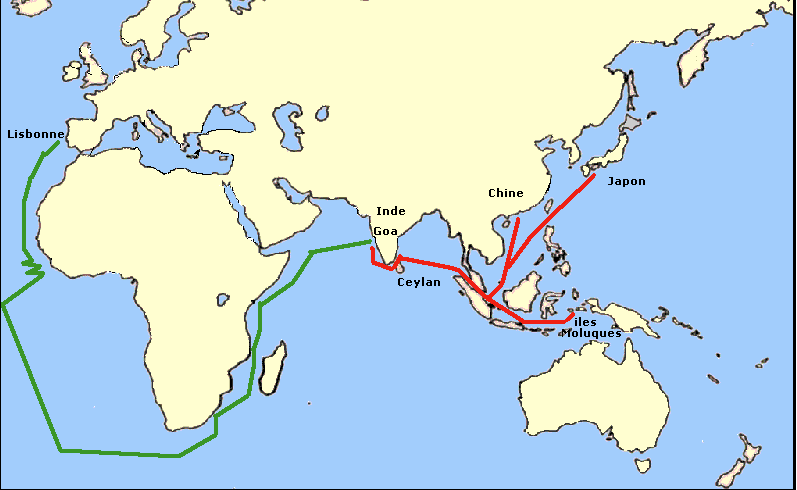
\includegraphics[width=\textwidth]{image/voyagesFrancoisXavier.png}
2.	Bibliographie

Eventuellement, notez l’ensemble des textes et références auxquels vous avez eu recours pour préparer l’exposé, y compris vos sources pour la biographie et les sites internet visités. 

3.	Nature du texte

Quel genre de texte est-ce (article, lettre, traité, sermon, etc..) ? Quel est son genre littéraire ?

4.	Le contexte historique et textuel

Situez la production du texte dans son contexte historique (date de la publication). A quelle occasion a-t-il été rédigé (suite à quel événement), dans quel contexte culturel et social, etc. ? A qui est-il adressé ?

Situez le texte dans son environnement littéraire, s’il est extrait d’un ouvrage ou d’un corpus. Présentez rapidement l’ouvrage, indiquez ce qui précède et ce qui suit le texte choisi, etc. Est-ce une traduction ?

5.	Si c’est un article de théologie


	5.1 La problématique 

Déterminer la problématique en vous inspirant des questions suivantes :
Après la phase de lecture pas à pas, vous construisez la question à laquelle l’auteur s’affronte :
-	pourquoi l’auteur se bat-il ?
-	quel problème essaie-t-il de régler, d’éclairer ? En général, il n’est pas difficile de trouver exposée la problématique en toute lettre dans le texte lui-même – parfois même de manière redondante ;
-	en fonction de quel contexte culturel, social, culturel, économique, politique l’auteur construit-il sa problématique ? Notez les événements déterminants auxquels il se réfère et les auteurs qu’il évoque – plus ou moins explicitement – comme ses alliés ou ses adversaires – et le cas échéant, renseignez-vous sur eux. 

5.2	 La thèse ou plutôt hypothèse

En fonction de la problématique de l’auteur, vous établissez la thèse (ou hypothèse) de l’article ou du texte étudié : quelle solution l’auteur apporte-t-il à sa question ? quelle perspective établit-il ? Là encore, il n’est pas difficile de trouver cette thèse exposée de manière explicite dans le texte lui-même. 

5.3	 L’argumentation 


Présentez la logique argumentative en fonction de laquelle l’auteur établit sa thèse (passe de l’hypothèse à la thèse vérifiée).

6.	Si c’est une lettre, une instruction ou un autre type de texte

	6.1 L’objet et l’effet recherché

Déterminer l’objet du texte et, éventuellement l’effet recherché (sur le lecteur).

6.2	 L’argumentation

Comment le texte mobilise-t-il des arguments, des images et des exemples pour toucher son lecteur ?

6.3	 Valeur théologique du texte

Quels sont les présupposés théologiques du texte ?


7.  Appréciation et discussion critique 

Critiquez le texte : l’argumentation est-elle convaincante ? Pourquoi ?
